% Options for packages loaded elsewhere
\PassOptionsToPackage{unicode}{hyperref}
\PassOptionsToPackage{hyphens}{url}
%
\documentclass[
]{book}
\usepackage{lmodern}
\usepackage{amssymb,amsmath}
\usepackage{ifxetex,ifluatex}
\ifnum 0\ifxetex 1\fi\ifluatex 1\fi=0 % if pdftex
  \usepackage[T1]{fontenc}
  \usepackage[utf8]{inputenc}
  \usepackage{textcomp} % provide euro and other symbols
\else % if luatex or xetex
  \usepackage{unicode-math}
  \defaultfontfeatures{Scale=MatchLowercase}
  \defaultfontfeatures[\rmfamily]{Ligatures=TeX,Scale=1}
\fi
% Use upquote if available, for straight quotes in verbatim environments
\IfFileExists{upquote.sty}{\usepackage{upquote}}{}
\IfFileExists{microtype.sty}{% use microtype if available
  \usepackage[]{microtype}
  \UseMicrotypeSet[protrusion]{basicmath} % disable protrusion for tt fonts
}{}
\makeatletter
\@ifundefined{KOMAClassName}{% if non-KOMA class
  \IfFileExists{parskip.sty}{%
    \usepackage{parskip}
  }{% else
    \setlength{\parindent}{0pt}
    \setlength{\parskip}{6pt plus 2pt minus 1pt}}
}{% if KOMA class
  \KOMAoptions{parskip=half}}
\makeatother
\usepackage{xcolor}
\IfFileExists{xurl.sty}{\usepackage{xurl}}{} % add URL line breaks if available
\IfFileExists{bookmark.sty}{\usepackage{bookmark}}{\usepackage{hyperref}}
\hypersetup{
  pdftitle={Notas de aulas de Estatística Econômica},
  pdfauthor={Marcos Minoru Hasegawa},
  hidelinks,
  pdfcreator={LaTeX via pandoc}}
\urlstyle{same} % disable monospaced font for URLs
\usepackage{color}
\usepackage{fancyvrb}
\newcommand{\VerbBar}{|}
\newcommand{\VERB}{\Verb[commandchars=\\\{\}]}
\DefineVerbatimEnvironment{Highlighting}{Verbatim}{commandchars=\\\{\}}
% Add ',fontsize=\small' for more characters per line
\usepackage{framed}
\definecolor{shadecolor}{RGB}{248,248,248}
\newenvironment{Shaded}{\begin{snugshade}}{\end{snugshade}}
\newcommand{\AlertTok}[1]{\textcolor[rgb]{0.94,0.16,0.16}{#1}}
\newcommand{\AnnotationTok}[1]{\textcolor[rgb]{0.56,0.35,0.01}{\textbf{\textit{#1}}}}
\newcommand{\AttributeTok}[1]{\textcolor[rgb]{0.77,0.63,0.00}{#1}}
\newcommand{\BaseNTok}[1]{\textcolor[rgb]{0.00,0.00,0.81}{#1}}
\newcommand{\BuiltInTok}[1]{#1}
\newcommand{\CharTok}[1]{\textcolor[rgb]{0.31,0.60,0.02}{#1}}
\newcommand{\CommentTok}[1]{\textcolor[rgb]{0.56,0.35,0.01}{\textit{#1}}}
\newcommand{\CommentVarTok}[1]{\textcolor[rgb]{0.56,0.35,0.01}{\textbf{\textit{#1}}}}
\newcommand{\ConstantTok}[1]{\textcolor[rgb]{0.00,0.00,0.00}{#1}}
\newcommand{\ControlFlowTok}[1]{\textcolor[rgb]{0.13,0.29,0.53}{\textbf{#1}}}
\newcommand{\DataTypeTok}[1]{\textcolor[rgb]{0.13,0.29,0.53}{#1}}
\newcommand{\DecValTok}[1]{\textcolor[rgb]{0.00,0.00,0.81}{#1}}
\newcommand{\DocumentationTok}[1]{\textcolor[rgb]{0.56,0.35,0.01}{\textbf{\textit{#1}}}}
\newcommand{\ErrorTok}[1]{\textcolor[rgb]{0.64,0.00,0.00}{\textbf{#1}}}
\newcommand{\ExtensionTok}[1]{#1}
\newcommand{\FloatTok}[1]{\textcolor[rgb]{0.00,0.00,0.81}{#1}}
\newcommand{\FunctionTok}[1]{\textcolor[rgb]{0.00,0.00,0.00}{#1}}
\newcommand{\ImportTok}[1]{#1}
\newcommand{\InformationTok}[1]{\textcolor[rgb]{0.56,0.35,0.01}{\textbf{\textit{#1}}}}
\newcommand{\KeywordTok}[1]{\textcolor[rgb]{0.13,0.29,0.53}{\textbf{#1}}}
\newcommand{\NormalTok}[1]{#1}
\newcommand{\OperatorTok}[1]{\textcolor[rgb]{0.81,0.36,0.00}{\textbf{#1}}}
\newcommand{\OtherTok}[1]{\textcolor[rgb]{0.56,0.35,0.01}{#1}}
\newcommand{\PreprocessorTok}[1]{\textcolor[rgb]{0.56,0.35,0.01}{\textit{#1}}}
\newcommand{\RegionMarkerTok}[1]{#1}
\newcommand{\SpecialCharTok}[1]{\textcolor[rgb]{0.00,0.00,0.00}{#1}}
\newcommand{\SpecialStringTok}[1]{\textcolor[rgb]{0.31,0.60,0.02}{#1}}
\newcommand{\StringTok}[1]{\textcolor[rgb]{0.31,0.60,0.02}{#1}}
\newcommand{\VariableTok}[1]{\textcolor[rgb]{0.00,0.00,0.00}{#1}}
\newcommand{\VerbatimStringTok}[1]{\textcolor[rgb]{0.31,0.60,0.02}{#1}}
\newcommand{\WarningTok}[1]{\textcolor[rgb]{0.56,0.35,0.01}{\textbf{\textit{#1}}}}
\usepackage{longtable,booktabs}
% Correct order of tables after \paragraph or \subparagraph
\usepackage{etoolbox}
\makeatletter
\patchcmd\longtable{\par}{\if@noskipsec\mbox{}\fi\par}{}{}
\makeatother
% Allow footnotes in longtable head/foot
\IfFileExists{footnotehyper.sty}{\usepackage{footnotehyper}}{\usepackage{footnote}}
\makesavenoteenv{longtable}
\usepackage{graphicx,grffile}
\makeatletter
\def\maxwidth{\ifdim\Gin@nat@width>\linewidth\linewidth\else\Gin@nat@width\fi}
\def\maxheight{\ifdim\Gin@nat@height>\textheight\textheight\else\Gin@nat@height\fi}
\makeatother
% Scale images if necessary, so that they will not overflow the page
% margins by default, and it is still possible to overwrite the defaults
% using explicit options in \includegraphics[width, height, ...]{}
\setkeys{Gin}{width=\maxwidth,height=\maxheight,keepaspectratio}
% Set default figure placement to htbp
\makeatletter
\def\fps@figure{htbp}
\makeatother
\setlength{\emergencystretch}{3em} % prevent overfull lines
\providecommand{\tightlist}{%
  \setlength{\itemsep}{0pt}\setlength{\parskip}{0pt}}
\setcounter{secnumdepth}{5}
\usepackage[brazil]{babel}
\usepackage[utf8]{inputenc}
\usepackage[T1]{fontenc}
\usepackage{lmodern}
\usepackage{amsmath,amssymb,amsthm,adjustbox,mathtools,bm,cool}
\usepackage{natbib}
\usepackage{graphics,graphicx,import,color,float}
\usepackage{url,booktabs,siunitx}
\usepackage[]{natbib}
\bibliographystyle{apalike}

\title{Notas de aulas de Estatística Econômica}
\author{Marcos Minoru Hasegawa}
\date{2020-09-29}

\begin{document}
\maketitle

{
\setcounter{tocdepth}{1}
\tableofcontents
}
\hypertarget{licenuxe7a}{%
\chapter*{Licença}\label{licenuxe7a}}
\addcontentsline{toc}{chapter}{Licença}

Como está descrito no repositório, os poucos códigos originais desenvolvidos ao longo do texto estão sob a licença \textbf{GNU GPLv3} .

O texto e as artes gráficas elaboradas de forma original estão sob licença \textbf{Creative Commons BY-NC-SA 4.0}.

\hypertarget{sobre-o-material}{%
\chapter*{Sobre o material}\label{sobre-o-material}}
\addcontentsline{toc}{chapter}{Sobre o material}

A situação especial causada pela pandemia da COVID-19 forçou a muitos professores criarem materiais para facilitar aulas remotas das suas disciplinas. A disciplina SE305 Estatística Econômica e Introdução à Econometria da UFPR não poderia ser diferente. Então, o objetivo deste material é de suprir a falta das bibliografias básicas na sua versão digital com a disponibilização de forma digital e gratuita o que seria o material das notas das aulas da disciplina de Estatística Econômica. Não é o ideal, mas a ideia é melhorar o material com tempo.

\hypertarget{sobre-o-autor}{%
\chapter*{Sobre o Autor}\label{sobre-o-autor}}
\addcontentsline{toc}{chapter}{Sobre o Autor}

Professor do Departamento de Economia da Universidade Federal do Paraná. Engenheiro Agrônomo pela UNESP/Jaboticabal, Mestrado em Economia Agrária pela ESALQ/USP e Doutorado em Economia Aplicada pela ESALQ/USP, é um dos professores responsáveis pelas disciplinas de SE305 Estatística Econômica e Introdução à Econometria e SE308 Econometria ambas do curso de Economia da Universidade Federal do Paraná (UFPR).

\hypertarget{estatuxedstica-descritiva}{%
\chapter{Estatística Descritiva}\label{estatuxedstica-descritiva}}

\hypertarget{medidas-de-posiuxe7uxe3o}{%
\section{Medidas de posição}\label{medidas-de-posiuxe7uxe3o}}

Este tópico está baseado no material de \citet{Sartoris2013}.

Trata-se de medidas de tendência central ou resumo. Como os nomes dizem, tratam-se de medidas que tratam de resumir a massa de valores e um único número.

\hypertarget{variuxe1vel-aleatuxf3ria}{%
\subsection{Variável Aleatória}\label{variuxe1vel-aleatuxf3ria}}

\begin{itemize}
\tightlist
\item
  variável aleatória (v.a.) é uma variável que está associada a uma \emph{distribuição de probabilidade}.
\item
  Ou seja, cada valor da v.a. está associada a uma probabilidade.
\item
  O resultado do lançamento de uma dado, que poder ser qualquer número de 1 a 6, está associada a uma probabilidade de \(1/6\).
\end{itemize}

\hypertarget{muxe9dia-aritmuxe9tica-simples}{%
\subsection{Média Aritmética Simples}\label{muxe9dia-aritmuxe9tica-simples}}

\begin{equation}
    \overline{X} = \frac{1}{n} \sum_{i=1}^{n} X_i
    \label{eq:mediaaritmeticasimples}
\end{equation}
onde \(i =1, ...,n\)

\textbf{Exemplo 1}

Qual é a média aritmética de um grupo de cinco pessoas cujas idades são em ordem crescente, 21,23,25,28 e 31. Para responder, basta aplicar \eqref{eq:mediaaritmeticasimples}.

\begin{equation*}
  \overline{X} = \frac{21+23+25+28+31}{5} = 25,6
\end{equation*}

\textbf{Exemplo 1 no R}

\begin{Shaded}
\begin{Highlighting}[]
\NormalTok{X <-}\StringTok{ }\KeywordTok{c}\NormalTok{(}\DecValTok{21}\NormalTok{, }\DecValTok{23}\NormalTok{, }\DecValTok{25}\NormalTok{, }\DecValTok{28}\NormalTok{, }\DecValTok{31}\NormalTok{)}
\NormalTok{X}
\end{Highlighting}
\end{Shaded}

\begin{verbatim}
## [1] 21 23 25 28 31
\end{verbatim}

\begin{Shaded}
\begin{Highlighting}[]
\NormalTok{mediaX <-}\StringTok{ }\KeywordTok{mean}\NormalTok{(X)}
\NormalTok{mediaX}
\end{Highlighting}
\end{Shaded}

\begin{verbatim}
## [1] 25,6
\end{verbatim}

\textbf{Exemplo 2}

Qual é a média aritmética de três provas realizadas por um aluno, cujas notas
foram 4,6 e 8. Para responder, basta aplicar \eqref{eq:mediaaritmeticasimples}.

\begin{equation*}
  \overline{X} = \frac{4+6+8}{3} = 6
\end{equation*}

\textbf{Exemplo 2 no R}

\begin{Shaded}
\begin{Highlighting}[]
\NormalTok{X2 <-}\StringTok{ }\KeywordTok{c}\NormalTok{(}\DecValTok{4}\NormalTok{, }\DecValTok{6}\NormalTok{, }\DecValTok{8}\NormalTok{)}
\NormalTok{X2}
\end{Highlighting}
\end{Shaded}

\begin{verbatim}
## [1] 4 6 8
\end{verbatim}

\begin{Shaded}
\begin{Highlighting}[]
\NormalTok{mediaX2 <-}\StringTok{ }\KeywordTok{mean}\NormalTok{(X2)}
\NormalTok{mediaX2}
\end{Highlighting}
\end{Shaded}

\begin{verbatim}
## [1] 6
\end{verbatim}

\hypertarget{muxe9dia-aritmuxe9tica-ponderada}{%
\subsection{Média Aritmética Ponderada}\label{muxe9dia-aritmuxe9tica-ponderada}}

Na média aritmética ponderada, cada valor pode ter importância diferentes do outros valores considerados no computo. A frequência dos valores é muito comumente usada para para dar maior ou menor importância relativa entre os valores considerados no computo da média aritmética ponderada. Veja como fica a fórmula para o cálculo da média aritmética ponderada em \eqref{eq:mediaartimeticaponderada}

\begin{equation}
    \overline{X} = \frac{1}{\sum_{i=1}^{n}w_i} \sum_{i=1}^{n} w_i X_i
    \label{eq:mediaartimeticaponderada}
\end{equation}
onde \(w_i\) é a ponderação ou peso associado a iésimo valor de \(X\).

Podemos escrever na forma de frequência relativa dos valores da variável \(X\):

\begin{equation}
  f_i = \frac{w_i}{\sum_{i=1}^{n}w_i}
  \label{eq:eq13}
\end{equation}

\textbf{Exemplo 3}

Qual é a média aritmética de um grupo de vinte alunos, oito com 22 anos, sete
de 23 anos, três de 25 anos, um de 28 anos e um de 30 anos. Para responder,
basta aplicar \eqref{eq:mediaartimeticaponderada}.

\begin{equation*}
  \overline{X} = \frac{22\times 8 + 23\times 7 + 25 \times 3 + 28 \times 1 + 
  30 \times 1}{20} = 23,5
\end{equation*}

\textbf{Exemplo 3 no R}

\begin{Shaded}
\begin{Highlighting}[]
\NormalTok{X3 <-}\StringTok{ }\KeywordTok{c}\NormalTok{(}\DecValTok{22}\NormalTok{, }\DecValTok{23}\NormalTok{, }\DecValTok{25}\NormalTok{, }\DecValTok{28}\NormalTok{, }\DecValTok{30}\NormalTok{)}
\NormalTok{X3}
\end{Highlighting}
\end{Shaded}

\begin{verbatim}
## [1] 22 23 25 28 30
\end{verbatim}

\begin{Shaded}
\begin{Highlighting}[]
\NormalTok{w3 <-}\StringTok{ }\KeywordTok{c}\NormalTok{(}\DecValTok{8}\NormalTok{, }\DecValTok{7}\NormalTok{, }\DecValTok{3}\NormalTok{, }\DecValTok{1}\NormalTok{, }\DecValTok{1}\NormalTok{)}
\NormalTok{w3}
\end{Highlighting}
\end{Shaded}

\begin{verbatim}
## [1] 8 7 3 1 1
\end{verbatim}

\begin{Shaded}
\begin{Highlighting}[]
\NormalTok{wX3 <-}\StringTok{ }\NormalTok{w3 }\OperatorTok{*}\StringTok{ }\NormalTok{X3}
\NormalTok{mediaX3 <-}\StringTok{ }\KeywordTok{sum}\NormalTok{(wX3)}\OperatorTok{/}\KeywordTok{sum}\NormalTok{(w3)}
\NormalTok{mediaX3}
\end{Highlighting}
\end{Shaded}

\begin{verbatim}
## [1] 23,5
\end{verbatim}

\textbf{Exemplo 4}

Qual é a média ponderada de três provas realizadas por um aluno, cujas notas foram 4, 6 e 8. A primeira prova tem peso igual a 1, a segunda tem peso igual a 2 e a terceira tem peso igual a 3. Para responder, basta aplicar \eqref{eq:mediaartimeticaponderada}.

\begin{equation*}
  \overline{X} = \frac{4 \times 1 + 6 \times 2 + 8 \times 3}{1 + 2 + 3} \cong 6,7
\end{equation*}

\textbf{Exemplo 4 no R}

\begin{Shaded}
\begin{Highlighting}[]
\NormalTok{X4 <-}\StringTok{ }\KeywordTok{c}\NormalTok{(}\DecValTok{4}\NormalTok{, }\DecValTok{6}\NormalTok{, }\DecValTok{8}\NormalTok{)}
\NormalTok{X4}
\end{Highlighting}
\end{Shaded}

\begin{verbatim}
## [1] 4 6 8
\end{verbatim}

\begin{Shaded}
\begin{Highlighting}[]
\NormalTok{w4 <-}\StringTok{ }\KeywordTok{c}\NormalTok{(}\DecValTok{1}\NormalTok{, }\DecValTok{2}\NormalTok{, }\DecValTok{3}\NormalTok{)}
\NormalTok{w4}
\end{Highlighting}
\end{Shaded}

\begin{verbatim}
## [1] 1 2 3
\end{verbatim}

\begin{Shaded}
\begin{Highlighting}[]
\NormalTok{wX4 <-}\StringTok{ }\NormalTok{w4 }\OperatorTok{*}\StringTok{ }\NormalTok{X4}
\NormalTok{mediaX4 <-}\StringTok{ }\KeywordTok{sum}\NormalTok{(wX4)}\OperatorTok{/}\KeywordTok{sum}\NormalTok{(w4)}
\KeywordTok{round}\NormalTok{(mediaX4, }\DataTypeTok{digits =} \DecValTok{1}\NormalTok{)}
\end{Highlighting}
\end{Shaded}

\begin{verbatim}
## [1] 6,7
\end{verbatim}

\hypertarget{muxe9dia-geomuxe9trica-simples}{%
\subsection{Média Geométrica Simples}\label{muxe9dia-geomuxe9trica-simples}}

Na média geométrica simples, a forma de obter uma medida resumo ou de tendência central é multiplicar todos os \(n\) valores e tirar a raiz enésima do resultado do produtório. Assim é possível ter duas fórmulas para a média geométrica a \eqref{eq:eq14} e \eqref{eq:eq15}.

\begin{equation}
    G = \left(\prod_{i=1}^{n} X_i \right)^{\frac{1}{n}}
    \label{eq:eq14}
\end{equation}
ou
\begin{equation}
    G = \sqrt[n]{X_1 \times X_2 \times \ldots \times X_n}
    \label{eq:eq15}
\end{equation}

O que acontece se um dos valores de \(X\) for igual a zero? E se um dos valores for negativo?

\textbf{Exemplo 5}

Sejam três valores 4, 6 e 8. Calcule a média geométrica simples.

\begin{equation*}
  \sqrt[3]{4 \times 6 \times 8} \cong 5,7690
\end{equation*}

\textbf{Exemplo 5 no R}

\begin{Shaded}
\begin{Highlighting}[]
\NormalTok{X5 <-}\StringTok{ }\KeywordTok{c}\NormalTok{(}\DecValTok{4}\NormalTok{, }\DecValTok{6}\NormalTok{, }\DecValTok{8}\NormalTok{)}
\NormalTok{X5}
\end{Highlighting}
\end{Shaded}

\begin{verbatim}
## [1] 4 6 8
\end{verbatim}

\begin{Shaded}
\begin{Highlighting}[]
\NormalTok{n <-}\StringTok{ }\KeywordTok{length}\NormalTok{(X5)}
\NormalTok{mediaX5 <-}\StringTok{ }\KeywordTok{prod}\NormalTok{(X5)}\OperatorTok{^}\NormalTok{(}\DecValTok{1}\OperatorTok{/}\NormalTok{n)}
\KeywordTok{round}\NormalTok{(mediaX5, }\DataTypeTok{digits =} \DecValTok{1}\NormalTok{)}
\end{Highlighting}
\end{Shaded}

\begin{verbatim}
## [1] 5,8
\end{verbatim}

\hypertarget{muxe9dia-geomuxe9trica-ponderada}{%
\subsection{Média Geométrica Ponderada}\label{muxe9dia-geomuxe9trica-ponderada}}

Na média geométrica ponderada que podem ser calculadas através de duas fórmulas \eqref{eq:eq16} e \eqref{eq:eq17}, cada valor pode ter uma importância diferente em relação aos outros valores no computo da média geométrica. Muito comumente, esta maior ou menor importância pode estar associada a frequência dos valores considerados no cálculo.

\begin{equation}
    G = \left(\prod_{j=1}^{k} X_j^{w_j} \right)^{\frac{1}{n}}
    \label{eq:eq16}
\end{equation}
ou
\begin{equation}
    G = \sqrt[n]{X_1^{w_1} \times X_2^{w_2} \times \ldots \times X_k^{w_k}}
    \label{eq:eq17}
\end{equation}

onde a \(\sum_{j=1}^{k} w_j = n\)

\textbf{Exemplo 6}

tomando os valores do exemplo 5 e ponderando por 1,2 e 3, temos:

\begin{equation*}
  \sqrt[6]{4^1 \times 6^2 \times 8^3} \cong 6,5
\end{equation*}

\textbf{O exemplo 6 no R}

\begin{Shaded}
\begin{Highlighting}[]
\NormalTok{x6 <-}\StringTok{ }\KeywordTok{c}\NormalTok{(}\DecValTok{4}\NormalTok{, }\DecValTok{6}\NormalTok{, }\DecValTok{8}\NormalTok{)}
\KeywordTok{class}\NormalTok{(x6)}
\end{Highlighting}
\end{Shaded}

\begin{verbatim}
## [1] "numeric"
\end{verbatim}

\begin{Shaded}
\begin{Highlighting}[]
\NormalTok{x6}
\end{Highlighting}
\end{Shaded}

\begin{verbatim}
## [1] 4 6 8
\end{verbatim}

\begin{Shaded}
\begin{Highlighting}[]
\NormalTok{w6 <-}\StringTok{ }\KeywordTok{c}\NormalTok{(}\DecValTok{1}\NormalTok{, }\DecValTok{2}\NormalTok{, }\DecValTok{3}\NormalTok{)}
\NormalTok{w6}
\end{Highlighting}
\end{Shaded}

\begin{verbatim}
## [1] 1 2 3
\end{verbatim}

\begin{Shaded}
\begin{Highlighting}[]
\NormalTok{G2 <-}\StringTok{ }\KeywordTok{round}\NormalTok{((}\KeywordTok{prod}\NormalTok{(x6}\OperatorTok{^}\NormalTok{w6))}\OperatorTok{^}\NormalTok{(}\DecValTok{1}\OperatorTok{/}\KeywordTok{sum}\NormalTok{(w6)), }\DecValTok{1}\NormalTok{)}
\NormalTok{G2}
\end{Highlighting}
\end{Shaded}

\begin{verbatim}
## [1] 6,5
\end{verbatim}

\hypertarget{muxe9dia-harmuxf4nica}{%
\subsection{Média Harmônica}\label{muxe9dia-harmuxf4nica}}

É o inverso da média dos inversos dos valores da variável que pode ser calculada através das fórmulas \eqref{eq:mediaharmonicasimples} e \eqref{eq:mediaharmonicasimples2}.

\begin{equation}
    H = \frac{n}{\sum_{i=1}^{n}\frac{1}{X_i}}
    \label{eq:mediaharmonicasimples}
\end{equation}

\begin{equation}
    H = \frac{n}{\frac{1}{X_1} + \frac{1}{X_2} + \ldots + \frac{1}{X_n}}
    \label{eq:mediaharmonicasimples2}
\end{equation}

O que acontece se um dos valores de \(X\) for igual a zero? Para entender essa situação, use o conceito de limite fazendo o valor tender a zero.

\textbf{Exemplo 7}

Tomando o exemplo das notas, temos:

\begin{equation*}
    H = \frac{3}{\frac{1}{4} + \frac{1}{6} + \frac{1}{8}}\cong 5,5.
\end{equation*}

\hypertarget{muxe9dia-harmuxf4nica-ponderada}{%
\subsection{Média Harmônica Ponderada}\label{muxe9dia-harmuxf4nica-ponderada}}

Na média harmônica ponderada, assim como na média aritmética ponderada e na média geométrica ponderada, cada valor pode ter uma importância em relação aos outros valores considerados no seu cálculo. Comumente, a frequência do valor pode associaar uma maior ou menor importância no cálculo da média harmônica ponderada que pode ser calculada através das fórmulas \eqref{eq:mediaharmonicaponderada} e \eqref{eq:mediaharmonicaponderada2}

\begin{equation}
    H = \frac{n}{\sum_{j=1}^{k}w_{j}\frac{1}{X_j}}
    \label{eq:mediaharmonicaponderada}
\end{equation}
ou
\begin{equation}
    H = \frac{n}{w_1\frac{1}{X_1} + w_2\frac{1}{X_2} + \ldots + w_k \frac{1}{X_k}}
    \label{eq:mediaharmonicaponderada2}
\end{equation}

onde a \(\sum_{j=1}^{k} w_j = n\)

\textbf{Exemplo 8}

Tomando o exemplo das notas

\begin{equation*}
    H = \frac{6}{\frac{1}{4}\times 1 + \frac{1}{6}\times 2 + \frac{1}{8}\times 3}\cong 6,3.
\end{equation*}

\textbf{Observação}

Tanto para as médias simples como para as ponderadas, a
média aritmética é maior do que a média geométrica e essa, por sua vez, é maior
que a harmônica. Isso só não vale quando todos os valores são iguais. Veja de forma esquemática em \eqref{eq:diferencaentreasmedias}

\begin{equation}
  \overline{X} \geq G \geq H
  \label{eq:diferencaentreasmedias}
\end{equation}

\textbf{Exemplo 9}

O aluno tira as seguintes notas bimestrais: 3,4,5,7 e 8,5. Determine qual seria sua média final se esta fosse calculada dos três modos, aritmética, geométirca e harmônica, em cada um dos seguintes casos: i) as notas têm o mesmo peso e; ii) as notas têm pesos diferentes.

\begin{enumerate}
\def\labelenumi{\roman{enumi})}
\tightlist
\item
  As notas dos bimestres têm os mesmos pesos.
\end{enumerate}

\begin{equation*}
    \overline{X} = \frac{3 + 4,5 + 7 + 8,5}{4} = 23/4 = 5,75
  \end{equation*}
\begin{equation*}
    G = \sqrt[4]{3 \times 4,5 \times 7 \times 8,5} = \sqrt[4]{803,25} \cong 5,32
  \end{equation*}
\begin{equation*}
    H = \frac{4}{\frac{1}{3} +\frac{1}{4,5} +\frac{1}{7} +\frac{1}{8,5}}   \cong 4,90
  \end{equation*}

\begin{enumerate}
\def\labelenumi{\roman{enumi})}
\setcounter{enumi}{1}
\tightlist
\item
  Suponha que agora os pesos para as notas bimestrais sejam, 30\%, 25\%, 25\% e 20\%.
\end{enumerate}

\begin{equation*}
    \overline{X} = 0,3\times 3 + 0,25\times 4,5 + 0,25\times 7 + 0,20 \times 8,5 = 5,475
  \end{equation*}
\begin{equation*}
    G = 3^{0,3} \times 4,5^{0,25} \times 7^{0,25} \times 8,5^{0,2} = \cong 5,05
  \end{equation*}
\begin{equation*}
    H = \frac{1}{0,3\frac{1}{3} +0,25\frac{1}{4,5} +0,25\frac{1}{7} +0,2\frac{1}{8,5}}   \cong 4,66
  \end{equation*}

\hypertarget{mediana}{%
\subsection{Mediana}\label{mediana}}

é o valor que divide um conjunto e dados ordenados ao meio, ou seja, dois
grupos de valores de igual tamanho. Com base na definição de mediana, o valor da mediana pode ser obtida através da sua posição que proporciona duas situações: i) o número de valores é impar e ii) o número de valores é par.

\begin{enumerate}
\def\labelenumi{\roman{enumi})}
\tightlist
\item
  Quando o número de valores é impar, a posiçãodo valor correspondente a mediana é obtida através de \eqref{eq:posicaomedianaimpar}:
\end{enumerate}

\begin{equation}
  PMediana_{impar} = \dfrac{n + 1}{2}
  \label{eq:posicaomedianaimpar}
\end{equation}
onde \(n\) é o número de valores considerado no cálculo.

\begin{enumerate}
\def\labelenumi{\roman{enumi})}
\setcounter{enumi}{1}
\tightlist
\item
  Quando o número de valores é par, a posição da mediana é obtida através da média entre os dois valores centrais do conjunto de valores ordenados de menor a maior. O primeiro valor central é definido pela posição obtida através de \eqref{eq:valor1mediaposicaomedianapar}
\end{enumerate}

\begin{equation}
  P1Mediana_{par} = \dfrac{n}{2}
  \label{eq:valor1mediaposicaomedianapar}
\end{equation}
onde \(n\) é o número de valores considerado para o cálculo.

O segundo valor central é definido pelas posição obtida através de
\eqref{eq:valor2mediaposicaomedianapar}

\begin{equation}
  P2Mediana_{par} = \dfrac{n}{2} + 1
  \label{eq:valor2mediaposicaomedianapar}
\end{equation}
onde \(n\) é o número de valores considerado para o cálculo.

Assim, a mediana quando o número de valores é par é obtida através da média aritmética simples dos valores correspondentes as posições obtidas por \eqref{eq:valor1mediaposicaomedianapar} e por
\eqref{eq:valor2mediaposicaomedianapar} através de \eqref{eq:medianapar}

\begin{equation}
  Mediana_{par} = \dfrac{ValorCentral_1 + ValorCentral_2}{2}
  \label{eq:medianapar}
\end{equation}

\textbf{Exemplo numérico de Mediana quando o número de valores é impar}

Seja um conjunto de valores 2,-3,1,-2,0,-1,3. Obtenha a mediana.

Primeiramente ordena-se do menor para o maior.

-3,-2,-1,0,1,2,3

Como se trata de número impar de valores o valor central que divide o conjunto de valores em dois subconjuntos de igual tamanho é o valor da mediana. Neste caso é o zero.

\textbf{Mediana no R}

\begin{Shaded}
\begin{Highlighting}[]
\NormalTok{w <-}\StringTok{ }\KeywordTok{c}\NormalTok{(}\OperatorTok{-}\DecValTok{3}\NormalTok{, }\DecValTok{-2}\NormalTok{, }\DecValTok{-1}\NormalTok{, }\DecValTok{0}\NormalTok{, }\DecValTok{1}\NormalTok{, }\DecValTok{2}\NormalTok{, }\DecValTok{3}\NormalTok{)}
\NormalTok{mediana1 <-}\StringTok{ }\KeywordTok{median}\NormalTok{(w)}
\KeywordTok{print}\NormalTok{(mediana1)}
\end{Highlighting}
\end{Shaded}

\begin{verbatim}
## [1] 0
\end{verbatim}

\textbf{Exemplo numérico de Mediana quando o número de valores é par}

No exemplo anterior o conjunto de dados era composto por um número ímpar de valores. Neste exemplo o número de valores ordenado de menor a maior é par. Nesse caso, apesar de existir vários critérios, o mais usual é tirar a média aritmética simples entre os dois valores centrais do conjunto de valores ordenados de menor a maior. Uma vez que não existe um valor que separe dois subconjuntos de igual tamanho, a média aritmética simples destes dois valores é o valor da mediana quando o número total de valores não é impar.

Sejam os valores -2,1,3,2,-3,1. Obtenha a mediana.

Primeiramente ordena-se os seis valores.

-3,-2,-1,1,2,3

Note que trata-se de conjunto com um número par de valores.

Dessa forma, toma-se os dois valores centrais que são -1 e 1 e calcula-se a média aritmética simples. Ou seja, a mediana para este conjunto com seis valores é igual a zero.

\textbf{O exemplo do número par de valores no R}

\begin{Shaded}
\begin{Highlighting}[]
\NormalTok{v <-}\StringTok{ }\KeywordTok{c}\NormalTok{(}\OperatorTok{-}\DecValTok{3}\NormalTok{, }\DecValTok{-2}\NormalTok{, }\DecValTok{-1}\NormalTok{, }\DecValTok{1}\NormalTok{, }\DecValTok{2}\NormalTok{, }\DecValTok{3}\NormalTok{)}
\NormalTok{mediana2 <-}\StringTok{ }\KeywordTok{median}\NormalTok{(v)}
\KeywordTok{print}\NormalTok{(mediana2)}
\end{Highlighting}
\end{Shaded}

\begin{verbatim}
## [1] 0
\end{verbatim}

\hypertarget{quartis-ou-quartiles}{%
\subsection{Quartis ou Quartiles}\label{quartis-ou-quartiles}}

são os valores que dividem o conjunto de dados ordenados em quatro subjconjuntos
de igual tamanho. Ou seja são valores do conjunto que definem o primeiro quarto
dos dados (25\%), a metade dos dados (50\%) que coincide com a mediana, os três
quartos dos dados (75\%).

Dessa forma para obter os valores que dividem o conjunto de dados ordenados de menor a maior e quatro subconjuntos de igual tamanho, é necessário definir qual é a posição desses valores. Uma vez definido as suas posições pode-se obter os valores corretamente.

A posição do valor que separa o primeiro do segundo quartil é definido por \eqref{eq:posicaoquartilum}.

\begin{equation}
  PQ_1 = \dfrac{(n +1)}{4}
  \label{eq:posicaoquartilum}
\end{equation}
onde \(n\) é o número de valores.
A posição do valor que separa o segundo do terceiro quartil é definido por \eqref{eq:posicaoquartiltres}.

\begin{equation}
  PQ_3 = \dfrac{3(n +1)}{4}
  \label{eq:posicaoquartiltres}
\end{equation}
onde \(n\) é o número de valores.

Note que o termo genérico é percentil. Por exemplo, o quintis são os valores que dividem o conjunto de ados ordenados de menor a maior em cinco subconjuntos de igual tamanho.

\textbf{Quartis no R}

No R tem uma função específica para a obtenção dos quartis.

\begin{Shaded}
\begin{Highlighting}[]
\NormalTok{p <-}\StringTok{ }\KeywordTok{c}\NormalTok{(}\DecValTok{0}\OperatorTok{:}\DecValTok{100}\NormalTok{)}
\KeywordTok{length}\NormalTok{(p)}
\end{Highlighting}
\end{Shaded}

\begin{verbatim}
## [1] 101
\end{verbatim}

\begin{Shaded}
\begin{Highlighting}[]
\KeywordTok{quantile}\NormalTok{(p)}
\end{Highlighting}
\end{Shaded}

\begin{verbatim}
##   0%  25%  50%  75% 100% 
##    0   25   50   75  100
\end{verbatim}

\begin{Shaded}
\begin{Highlighting}[]
\NormalTok{faixainterquant <-}\StringTok{ }\KeywordTok{quantile}\NormalTok{(p, }\FloatTok{0.75}\NormalTok{) }\OperatorTok{-}\StringTok{ }\KeywordTok{quantile}\NormalTok{(p, }
    \FloatTok{0.25}\NormalTok{)}
\NormalTok{faixainterquant}
\end{Highlighting}
\end{Shaded}

\begin{verbatim}
## 75% 
##  50
\end{verbatim}

\textbf{Quartis no R}

No R tem uma função específica para a obtenção dos quartis.

\begin{Shaded}
\begin{Highlighting}[]
\NormalTok{p2 <-}\StringTok{ }\KeywordTok{c}\NormalTok{(}\DecValTok{1}\OperatorTok{:}\DecValTok{100}\NormalTok{)}
\KeywordTok{length}\NormalTok{(p2)}
\end{Highlighting}
\end{Shaded}

\begin{verbatim}
## [1] 100
\end{verbatim}

\begin{Shaded}
\begin{Highlighting}[]
\KeywordTok{quantile}\NormalTok{(p2)}
\end{Highlighting}
\end{Shaded}

\begin{verbatim}
##     0%    25%    50%    75%   100% 
##   1,00  25,75  50,50  75,25 100,00
\end{verbatim}

\begin{Shaded}
\begin{Highlighting}[]
\NormalTok{faixainterquant2 <-}\StringTok{ }\KeywordTok{quantile}\NormalTok{(p2, }\FloatTok{0.75}\NormalTok{) }\OperatorTok{-}\StringTok{ }\KeywordTok{quantile}\NormalTok{(p2, }
    \FloatTok{0.25}\NormalTok{)}
\NormalTok{faixainterquant2}
\end{Highlighting}
\end{Shaded}

\begin{verbatim}
##  75% 
## 49,5
\end{verbatim}

\hypertarget{moda}{%
\subsection{Moda}\label{moda}}

\textbf{Moda} é o elemento de maior frequência, ou seja, que aparece o maior número de vezes. Pode haver mais de uma moda em um conjunto de valores:

\begin{itemize}
\tightlist
\item
  Unimodal
\item
  Bimodal
\item
  Multimodal
\item
  Amodal
\end{itemize}

\textbf{Moda no R}
Não existe uma função da moda para pronto uso no R. É necessário criar uma função
segue abaixo.

\begin{Shaded}
\begin{Highlighting}[]
\CommentTok{# criando a função moda no R}

\NormalTok{getmode <-}\StringTok{ }\ControlFlowTok{function}\NormalTok{(v) \{}
\NormalTok{    uniqv <-}\StringTok{ }\KeywordTok{unique}\NormalTok{(v)}
\NormalTok{    uniqv[}\KeywordTok{which.max}\NormalTok{(}\KeywordTok{tabulate}\NormalTok{(}\KeywordTok{match}\NormalTok{(v, uniqv)))]}
\NormalTok{\}}
\NormalTok{z <-}\StringTok{ }\KeywordTok{c}\NormalTok{(}\DecValTok{2}\NormalTok{, }\DecValTok{1}\NormalTok{, }\DecValTok{2}\NormalTok{, }\DecValTok{3}\NormalTok{, }\DecValTok{1}\NormalTok{, }\DecValTok{2}\NormalTok{, }\DecValTok{3}\NormalTok{, }\DecValTok{4}\NormalTok{, }\DecValTok{1}\NormalTok{, }\DecValTok{5}\NormalTok{, }\DecValTok{5}\NormalTok{, }\DecValTok{3}\NormalTok{, }\DecValTok{2}\NormalTok{, }\DecValTok{3}\NormalTok{)}
\NormalTok{moda1 <-}\StringTok{ }\KeywordTok{getmode}\NormalTok{(z)}
\KeywordTok{print}\NormalTok{(moda1)}
\end{Highlighting}
\end{Shaded}

\begin{verbatim}
## [1] 2
\end{verbatim}

\hypertarget{medidas-de-dispersuxe3o}{%
\section{Medidas de dispersão}\label{medidas-de-dispersuxe3o}}

Este tópico está baseado nos materiais de \citet{Hoffmann2006}, \citet{Morettin2013} e \citet{Sartoris2013}.

Medem como os dados estão \textit{agrupados}, mais ou menos próximos entre si,
seja, mais ou menos dispersos.

\hypertarget{amplitude}{%
\subsection{Amplitude}\label{amplitude}}

A amplitude de um conjunto de valores é a diferença entre o maior elemento e o menor elemento desse conjunto.

\hypertarget{variuxe2ncia}{%
\subsection{Variância}\label{variuxe2ncia}}

A variância é a somatória dos quadrados dos desvios em relação a média, dividido pelo número de observações. Note que a ideia inicial de dispersão foi a distância de cada valor do conjunto dados da variável em relação à media da variável. Mas como trata-se da distância relativa de cada valor em relação a média dos valores da variável, a sua somatória sempre resulta zero. Pois os desvios em relação a médias são compostos de valores positivos e negativos por estarem acima ou abaixo da média e assim a somatória das mesmas resulta zero, sempre. Portanto, a soma dos desvios não tem utilidade como medida de dispersão. Mas se a soma for dos quadrados dos desvios, isso é resolvido. Por isso, a variância é o valor médio dos quadrados dos desvios em relação à media. Ou seja,

\begin{equation*}
  var(X) =\sigma^2 = \frac{\sum_{i=1}^{n}(X_i - \overline{X})^2}{n}~\text{(população)}
\end{equation*}

\begin{equation*}
  var(X) =\sigma^2 = \frac{\sum_{i=1}^{n}(X_i - \overline{X})^2}{n-1}~\text{(amostra)}
\end{equation*}

Note que a variância da amostra é um estimador não viesado da variância populacional. A diferença entre variância populacional e variância amostral será apresentada mais adiante. A interpretação intuitiva da diferença entre ambas as variâncias é de que quando se trabalha com amostra, está tendo acesso a parte das informações e isso precisa ser penalizado. Note que esta penalização se dá para amostras pequenas pois se trata de subtrair uma unidade do número de observações.
O que acontece com a diferença entre variância populacional e a variância amostral quando i) o número de observações torna-se muito grande, tipo bem maior que 30 e; ii) o número de observações tende ao infinito.

\textbf{Variância no R}

Aproveitando os dados de alturas de 30 pessoas:

\begin{Shaded}
\begin{Highlighting}[]
\KeywordTok{tail}\NormalTok{(X)}
\end{Highlighting}
\end{Shaded}

\begin{verbatim}
## [1] 21 23 25 28 31
\end{verbatim}

\begin{Shaded}
\begin{Highlighting}[]
\NormalTok{varX <-}\StringTok{ }\KeywordTok{round}\NormalTok{(}\KeywordTok{var}\NormalTok{(X), }\DecValTok{4}\NormalTok{)}
\NormalTok{varX}
\end{Highlighting}
\end{Shaded}

\begin{verbatim}
## [1] 15,8
\end{verbatim}

Note que a variância no R é a variância amostral, cujo denominador é \((n-1)\).

Em termos práticos, a variância tem uma desvantagem: a unidade do seu resultado é o quadrado da unidade original da variável. Portanto, se a variável em questão é preço de uma mercadoria em Reais, a sua variância será Reais ao quadrado. Tal fato dificulta a sua interpretação. Por isso é apresentado o desvio padrão como medida de dispersão na sequência.

\hypertarget{desvio-padruxe3o}{%
\subsection{Desvio Padrão}\label{desvio-padruxe3o}}

É a raiz quadrada da variância. No desvio padrão, denotado como \(d.p.(X)\) ou
\(\sigma\), não tem o efeito do quadrado.

\begin{equation*}
  d.p.(X) \cong \sigma = \sqrt{var(X)}
\end{equation*}

Portanto, a sua interpretação é clara e direta por ter a mesma unidade da sua variável original. Desta forma, o desvio padrão facilita a sua análise juntamente com as medidas de posição como a média aritmética simples, por exemplo.

\textbf{Desvio Padrão no R}

\begin{Shaded}
\begin{Highlighting}[]
\KeywordTok{tail}\NormalTok{(X)}
\end{Highlighting}
\end{Shaded}

\begin{verbatim}
## [1] 21 23 25 28 31
\end{verbatim}

\begin{Shaded}
\begin{Highlighting}[]
\NormalTok{dpX <-}\StringTok{ }\KeywordTok{round}\NormalTok{(}\KeywordTok{sd}\NormalTok{(X), }\DecValTok{4}\NormalTok{)}
\NormalTok{dpX}
\end{Highlighting}
\end{Shaded}

\begin{verbatim}
## [1] 3,9749
\end{verbatim}

Note que, da mesma forma que a variância no R, o desvio padrão calculado no R tem como base a variância cujo numerador é \((n-1)\).

\textbf{Fórmula alternativa da Variância}

Desenvolvendo a fórmula da definição da variância tem-se:
\begin{align*}
  var(X)  &= \frac{1}{n}\sum_{i=1}^{n}(X_i - \overline{X})^2 \\
          &= \frac{1}{n}\sum_{i=1}^{n}(X_i^2 - 2X_i\overline{X} +
          \overline{X}^2)\\
          &= \frac{1}{n}\sum_{i=1}^{n}X_i^2 - 
          \frac{1}{n}\sum_{i=1}^{n}2X_i\overline{X}+
          \frac{1}{n}\sum_{i=1}^{n}\overline{X}^2\\
          &= \frac{1}{n}\sum_{i=1}^{n}X_i^2 - 
          2\overline{X}\frac{1}{n}\sum_{i=1}^{n}X_i+
          \frac{1}{n}n\overline{X}^2\\
          &= \frac{1}{n}\sum_{i=1}^{n}X_i^2 - 
          2\overline{X}\overline{X}+ \overline{X}^2\\
          &= \frac{1}{n}\sum_{i=1}^{n}X_i^2 - \overline{X}^2.
\end{align*}

Em outras palavras

\begin{equation*}
  var(X) = \text{média dos quadrados} - \text{quadrado da média}.
\end{equation*}

\textbf{Exemplo de variância e desvio padrão no R}

Tomando o exemplo numérico da tabela 2.7 (Sartoris, 2013, p.40) sobre notas do
aluno A tem-se:

\begin{longtable}[]{@{}lcc@{}}
\toprule
Aluno A & notas & \(notas^2\)\tabularnewline
\midrule
\endhead
Economia & 3 & 9\tabularnewline
Contabilidade & 2 & 4\tabularnewline
Administração & 4 & 16\tabularnewline
Matemática & 1 & 1\tabularnewline
\textbf{Somatória} & \textbf{10} & \textbf{30}\tabularnewline
\textbf{Média} & \textbf{2,5} & \textbf{7,5}\tabularnewline
\bottomrule
\end{longtable}

\begin{equation*}
  var(X) = 7,5 - (2,5)^2 = 1,25
\end{equation*}

\begin{equation*}
  dp(X) = \sqrt{1,25} = 1,12
\end{equation*}

\begin{Shaded}
\begin{Highlighting}[]
\NormalTok{X3 <-}\StringTok{ }\KeywordTok{c}\NormalTok{(}\DecValTok{3}\NormalTok{, }\DecValTok{2}\NormalTok{, }\DecValTok{4}\NormalTok{, }\DecValTok{1}\NormalTok{)}
\NormalTok{mediaX3e2 <-}\StringTok{ }\KeywordTok{sum}\NormalTok{(X3}\OperatorTok{^}\DecValTok{2}\NormalTok{)}\OperatorTok{/}\KeywordTok{length}\NormalTok{(X3)}
\NormalTok{mediaX3 <-}\StringTok{ }\KeywordTok{sum}\NormalTok{(X3)}\OperatorTok{/}\KeywordTok{length}\NormalTok{(X3)}
\NormalTok{varX3 <-}\StringTok{ }\NormalTok{mediaX3e2 }\OperatorTok{-}\StringTok{ }\NormalTok{mediaX3}\OperatorTok{^}\DecValTok{2}
\NormalTok{varX3}
\end{Highlighting}
\end{Shaded}

\begin{verbatim}
## [1] 1,25
\end{verbatim}

\begin{Shaded}
\begin{Highlighting}[]
\NormalTok{dpX3 <-}\StringTok{ }\KeywordTok{round}\NormalTok{(}\KeywordTok{sqrt}\NormalTok{(varX3), }\DecValTok{4}\NormalTok{)}
\NormalTok{dpX3}
\end{Highlighting}
\end{Shaded}

\begin{verbatim}
## [1] 1,118
\end{verbatim}

\hypertarget{desvio-absoluto-muxe9dio}{%
\subsection{Desvio Absoluto Médio}\label{desvio-absoluto-muxe9dio}}

\hypertarget{diferenuxe7a-muxe9dia}{%
\subsection{Diferença Média}\label{diferenuxe7a-muxe9dia}}

\hypertarget{histograma}{%
\subsection{Histograma}\label{histograma}}

O histograma é uma ferramenta da estatística descritiva para mostrar visualmente, de forma bastante simples, como os valores da variável estão distribuídos. Mas também permite ter uma ideia visual da dispersão do conjunto de valores. Portanto, não se trata de uma medida de dispersão. Mas deveria ser a primeira coisa a se obter das variáveis de interesse em um trabalho de pesquisa.

Considere a altura de 30 pessoas medidas em centímetros.

Tabela 2.1 - Altura de 30 pessoas em cm.

\begin{longtable}[]{@{}ccccc@{}}
\toprule
\endhead
159 & 168 & 172 & 175 & 181\tabularnewline
161 & 168 & 173 & 176 & 183\tabularnewline
162 & 169 & 173 & 177 & 185\tabularnewline
164 & 170 & 174 & 178 & 190\tabularnewline
166 & 171 & 174 & 179 & 194\tabularnewline
167 & 171 & 174 & 180 & 201\tabularnewline
\bottomrule
\end{longtable}

\textbf{Usando o R para construir o histograma do exemplo numérico}

Os dados são inputados na variável X.

\begin{Shaded}
\begin{Highlighting}[]
\NormalTok{X <-}\StringTok{ }\KeywordTok{c}\NormalTok{(}\DecValTok{159}\NormalTok{, }\DecValTok{161}\NormalTok{, }\DecValTok{162}\NormalTok{, }\DecValTok{164}\NormalTok{, }\DecValTok{166}\NormalTok{, }\DecValTok{167}\NormalTok{, }\DecValTok{168}\NormalTok{, }\DecValTok{168}\NormalTok{, }\DecValTok{169}\NormalTok{, }
    \DecValTok{170}\NormalTok{, }\DecValTok{171}\NormalTok{, }\DecValTok{171}\NormalTok{, }\DecValTok{172}\NormalTok{, }\DecValTok{173}\NormalTok{, }\DecValTok{173}\NormalTok{, }\DecValTok{174}\NormalTok{, }\DecValTok{174}\NormalTok{, }\DecValTok{174}\NormalTok{, }\DecValTok{175}\NormalTok{, }
    \DecValTok{176}\NormalTok{, }\DecValTok{177}\NormalTok{, }\DecValTok{178}\NormalTok{, }\DecValTok{179}\NormalTok{, }\DecValTok{180}\NormalTok{, }\DecValTok{181}\NormalTok{, }\DecValTok{183}\NormalTok{, }\DecValTok{185}\NormalTok{, }\DecValTok{190}\NormalTok{, }\DecValTok{194}\NormalTok{, }
    \DecValTok{201}\NormalTok{)}
\KeywordTok{head}\NormalTok{(X)}
\end{Highlighting}
\end{Shaded}

\begin{verbatim}
## [1] 159 161 162 164 166 167
\end{verbatim}

\begin{Shaded}
\begin{Highlighting}[]
\NormalTok{obsX <-}\StringTok{ }\KeywordTok{length}\NormalTok{(X)}
\NormalTok{obsX}
\end{Highlighting}
\end{Shaded}

\begin{verbatim}
## [1] 30
\end{verbatim}

\begin{Shaded}
\begin{Highlighting}[]
\NormalTok{faixaX <-}\StringTok{ }\KeywordTok{range}\NormalTok{(X)}
\NormalTok{faixaX}
\end{Highlighting}
\end{Shaded}

\begin{verbatim}
## [1] 159 201
\end{verbatim}

\textbf{Usando a função hist do R para elaborar o histograma de altura}

\begin{Shaded}
\begin{Highlighting}[]
\NormalTok{grafico1 <-}\StringTok{ }\KeywordTok{hist}\NormalTok{( }
\NormalTok{                  X, }
                  \DataTypeTok{main=}\StringTok{"Histograma da Altura"}\NormalTok{, }
                  \DataTypeTok{xlab=}\StringTok{"cm"}\NormalTok{, }
                  \DataTypeTok{ylab=}\StringTok{"frequência", }
\StringTok{                  border="}\NormalTok{blue}\StringTok{", }
\StringTok{                  col="}\NormalTok{green}\StringTok{", }
\StringTok{                  xlim=c(150,210), }
\StringTok{                  las=1, }
\StringTok{                  breaks=5, }
\StringTok{                  right=FALSE }
\StringTok{                ) }

\StringTok{grafico1}
\end{Highlighting}
\end{Shaded}

onde

\begin{itemize}
\tightlist
\item
  \textbf{main=``Histograma da Altura de 30 pessoas''} titulo do histograma
\item
  \textbf{xlab=``cm''} rotulo do eixo horizontal
\item
  \textbf{ylab=``frequência''} rotulo do eixo vertical
\item
  \textbf{border=``blue''} cor do contorno das barras
\item
  \textbf{col=``green''} cor das barras
\item
  \textbf{xlim=c(150,210)} limite inferior e superior
\item
  \textbf{las=1} rotacao do rotulo dos numeros do eixo vertical
\item
  \textbf{breaks=5} número de classes
\item
  \textbf{right=FALSE} define intervalo do tipo {[}a,b), se FALSE, e (a,b{]}, se TRUE.
\end{itemize}

\textbf{Obtendo o histograma}

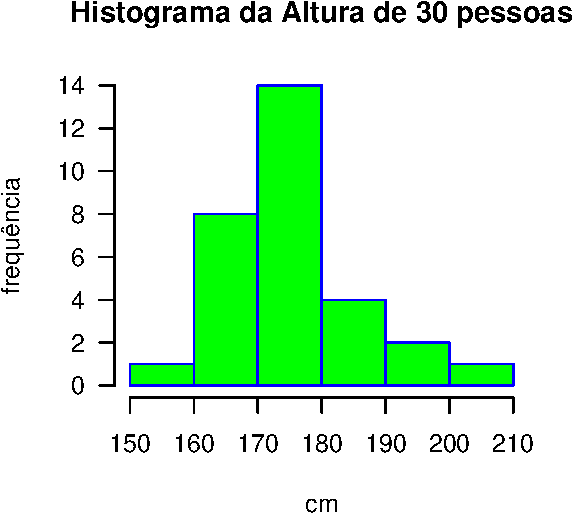
\includegraphics{EstatEcon_files/figure-latex/histograma12-1.pdf}

O pacote \textbf{ggplot2} gera gráficos e histogramas melhor elaborados.

\textbf{Obtendo o histograma usando uma forma alternativa}

Agrupando essas pessoas em \textbf{classes} de 10 cm temos:

\begin{longtable}[]{@{}cc@{}}
\toprule
classes & frequência\tabularnewline
\midrule
\endhead
{[}150 ; 160{[} & 1\tabularnewline
{[}160 ; 170{[} & 8\tabularnewline
{[}170 ; 180{[} & 14\tabularnewline
{[}180 ; 190{[} & 4\tabularnewline
{[}190 ; 200{[} & 2\tabularnewline
{[}200 ; 210{[} & 1\tabularnewline
\bottomrule
\end{longtable}

Fazendo isso no R:

\begin{Shaded}
\begin{Highlighting}[]
\NormalTok{nobs <-}\StringTok{ }\KeywordTok{c}\NormalTok{(}\DecValTok{1}\OperatorTok{:}\DecValTok{30}\NormalTok{)}
\NormalTok{dataX <-}\StringTok{ }\KeywordTok{as.data.frame}\NormalTok{(}\KeywordTok{cbind}\NormalTok{(nobs, X))}
\CommentTok{# transformando em data frame}
\KeywordTok{tail}\NormalTok{(dataX)}
\end{Highlighting}
\end{Shaded}

\begin{verbatim}
##    nobs   X
## 25   25 181
## 26   26 183
## 27   27 185
## 28   28 190
## 29   29 194
## 30   30 201
\end{verbatim}

\begin{Shaded}
\begin{Highlighting}[]
\CommentTok{# mostrando as seis últimas observações}
\NormalTok{quebras <-}\StringTok{ }\KeywordTok{seq}\NormalTok{(}\DecValTok{150}\NormalTok{, }\DecValTok{210}\NormalTok{, }\DataTypeTok{by =} \DecValTok{10}\NormalTok{)}
\CommentTok{# definindo os intervalos}
\NormalTok{quebras}
\end{Highlighting}
\end{Shaded}

\begin{verbatim}
## [1] 150 160 170 180 190 200 210
\end{verbatim}

\begin{Shaded}
\begin{Highlighting}[]
\NormalTok{dataX.cut <-}\StringTok{ }\KeywordTok{cut}\NormalTok{(dataX}\OperatorTok{$}\NormalTok{X, quebras, }\DataTypeTok{right =} \OtherTok{FALSE}\NormalTok{)}
\CommentTok{# construindo as classes fechado a esq e aberto a}
\CommentTok{# direita}
\NormalTok{dataX.freq <-}\StringTok{ }\KeywordTok{table}\NormalTok{(dataX.cut)}
\CommentTok{# obtendo a frequência para cada classe.}
\NormalTok{dataXfreq <-}\StringTok{ }\KeywordTok{cbind}\NormalTok{(dataX.freq)}
\CommentTok{# colocando os dados em colunas}
\NormalTok{dataXfreq}
\end{Highlighting}
\end{Shaded}

\begin{verbatim}
##           dataX.freq
## [150,160)          1
## [160,170)          8
## [170,180)         14
## [180,190)          4
## [190,200)          2
## [200,210)          1
\end{verbatim}

\hypertarget{diagrama-de-caixa-boxplot}{%
\subsection{Diagrama de caixa (Boxplot)}\label{diagrama-de-caixa-boxplot}}

O texto sobre o diagrama de caixa foi baseado em \citet{Morettin2013}.

Boxplot ou caixa de bigode também é uma ferramenta da estatística descritva que permite visualizar a dispersão dos valores da variável em análise. O que define o diagrama de caixa são os quartis. A parte inferior e superior da caixa, são respectivamente o primeiro quartil (\(Q_1\)) e o terceiro quartil (\(Q_3\)). A linha que corta da caixa é a mediana ou o segundo quartil (\(Q_2\)). Os bigodes que são as linhas que se estendem a partir da caixa, são calculado com base na amplitude interquartil (\(AIQ\)). A amplitude interquartil é a diferença entre os valores do terceiro e do primeiro quartis. Ou seja,

\begin{equation*}
  AIQ = Q_3 - Q_1
\end{equation*}

O bigode inferior denominado \(LI\) é calculado subtraindo \(1,5\times AIQ\) do valor do primeiro quartil \(Q_1\). Ou seja,

\begin{equation*}
  LI = Q_1 - 1,5 \times AIQ
\end{equation*}

O bigode superior, denominado \(LS\), é calculado somando \(1,5\times AIQ\) ao valor da terceiro quartil \(Q_3\). Ou seja,

\begin{equation*}
  LS = Q_1 + 1,5 \times AIQ
\end{equation*}

Os valores que forem menor que o \(LI\) ou maior que o \(LS\) são denominados valores discrepantes oui \emph{outliers}. Os valores discrepantes, quando existentes, são colocados separadamente no diagrama de caixa mantendo a distancia relativa do limite inferior ou do limite superior.

Toma-se o mesmo exemplo da altura de 30 pessoas para apresentar o boxplot.

O código seria:

\begin{Shaded}
\begin{Highlighting}[]
\KeywordTok{boxplot}\NormalTok{(X, }\DataTypeTok{data =}\NormalTok{ dataX, }\DataTypeTok{main =} \StringTok{"Diagrama de Caixa"}\NormalTok{, }
    \DataTypeTok{ylab =} \StringTok{"cm"}\NormalTok{, }\DataTypeTok{xlab =} \StringTok{"altura de 30 pessoas"}\NormalTok{)}
\end{Highlighting}
\end{Shaded}

e o resultado segue abaixo.

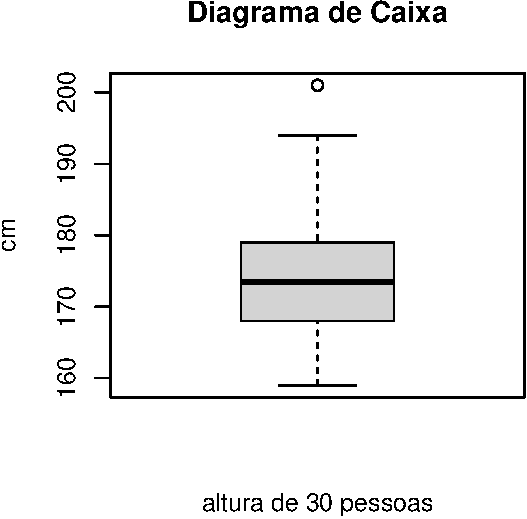
\includegraphics{EstatEcon_files/figure-latex/diagrama de caixa12-1.pdf}

\hypertarget{medidas-de-relauxe7uxe3o-linear-entre-duas-variuxe1veis}{%
\section{Medidas de relação linear entre duas variáveis}\label{medidas-de-relauxe7uxe3o-linear-entre-duas-variuxe1veis}}

Este assunto tem como base o material de \citet{Sartoris2013}.

Parece um pouco estranho incluir esse tópico logo depois das medidas de dispersão. Mas a variância é um caso especial da covariância que é a primeira medida de relação linear entre duas variáveis.

O coeficiente de correlação utiliza a covariância e o desvio padrão para resolver o problema de interpretação do resultado da covariância.

\hypertarget{covariuxe2ncia}{%
\subsection{Covariância}\label{covariuxe2ncia}}

pode ser estendida como uma \emph{variância conjunta} entre duas variáveis. Ou seja,
\begin{equation*}
  cov(X,Y) = \frac{1}{n}\sum_{i=1}^{n}(X_i - \overline{X})(Y_i - \overline{Y})
\end{equation*}

\textbf{Fórmula alternativa da Variância}

Também existe a fórmula alternativa da covariância.

\begin{equation*}
  cov(X,Y) = \frac{1}{n}\sum_{i=1}^{n}X_{i}Y_{i} - \overline{X}\overline{Y}.
\end{equation*}

\textbf{Fórmula alternativa da Covariância}

Em outras palavras

\begin{equation*}
  cov(X,Y) = \text{média dos produtos de X e Y} - \text{produto das médias de X e Y}.
\end{equation*}

\textbf{Covariância no R}

Tomando o exemplo de consumo e renda da tabela 2.11 (Sartoris, 2013, p.42) tem-se

\begin{longtable}[]{@{}cccc@{}}
\toprule
Ano & Consumo(X) & Renda(Y) & (XY)\tabularnewline
\midrule
\endhead
1 & 600 & 1.000 & 600.000\tabularnewline
2 & 700 & 1.100 & 770.000\tabularnewline
3 & 800 & 1.300 & 1.040.000\tabularnewline
4 & 900 & 1.400 & 1.260.000\tabularnewline
\textbf{Somatória} & \textbf{3.000} & \textbf{4.800} & \textbf{3.670.000}\tabularnewline
\textbf{Média} & \textbf{750} & \textbf{1.200} & \textbf{917.500}\tabularnewline
\bottomrule
\end{longtable}

\textbf{Covariância no R}

\begin{Shaded}
\begin{Highlighting}[]
\NormalTok{C1 <-}\StringTok{ }\KeywordTok{c}\NormalTok{(}\DecValTok{600}\NormalTok{, }\DecValTok{700}\NormalTok{, }\DecValTok{800}\NormalTok{, }\DecValTok{900}\NormalTok{)}
\NormalTok{R1 <-}\StringTok{ }\KeywordTok{c}\NormalTok{(}\DecValTok{1000}\NormalTok{, }\DecValTok{1100}\NormalTok{, }\DecValTok{1300}\NormalTok{, }\DecValTok{1400}\NormalTok{)}
\NormalTok{mediaC1 <-}\StringTok{ }\KeywordTok{sum}\NormalTok{(C1)}\OperatorTok{/}\KeywordTok{length}\NormalTok{(C1)}
\NormalTok{mediaR1 <-}\StringTok{ }\KeywordTok{sum}\NormalTok{(R1)}\OperatorTok{/}\KeywordTok{length}\NormalTok{(R1)}
\NormalTok{mediaC1R1 <-}\StringTok{ }\KeywordTok{sum}\NormalTok{(C1 }\OperatorTok{*}\StringTok{ }\NormalTok{R1)}\OperatorTok{/}\KeywordTok{length}\NormalTok{(C1)}
\NormalTok{covC1R1 <-}\StringTok{ }\NormalTok{mediaC1R1 }\OperatorTok{-}\StringTok{ }\NormalTok{mediaC1 }\OperatorTok{*}\StringTok{ }\NormalTok{mediaR1}
\NormalTok{covC1R1}
\end{Highlighting}
\end{Shaded}

\begin{verbatim}
## [1] 17500
\end{verbatim}

\begin{Shaded}
\begin{Highlighting}[]
\KeywordTok{cov}\NormalTok{(C1, R1)}
\end{Highlighting}
\end{Shaded}

\begin{verbatim}
## [1] 23333,33
\end{verbatim}

Note que a função covariância no R é calculada dividindo por \((n-1)\) e não por \(n\).

\hypertarget{coeficiente-de-correlauxe7uxe3o}{%
\subsection{Coeficiente de Correlação}\label{coeficiente-de-correlauxe7uxe3o}}

É obtido dividindo a covariância pelos desvios padrões das variáveis, retirando-se o efeito dos valores de cada variável. Como as unidades das variáveis se cancelam matematicamente, o coeficiente de correlação é um número puro que varia entre -1 e +1. Essa característica o torna mais fácil e claro a sua interpretação. Ou seja,

\begin{equation*}
 corr(X,Y) \cong \rho_{xy} = \frac{cov(X,Y)}{dp(X) \times dp(Y)}
\end{equation*}
onde
\begin{equation*}
  -1 \leq \rho \leq +1
\end{equation*}

Portanto, quando o coeficiente de correlação é igual a zero ou muito próximo a zero, significa que as duas variáveis analisadas não tem relação do tipo linear entre elas. Quando a o coeficiente de correlação é igual a -1 ou próximo de -1, tal fato indica que a existência de uma relação do tipo linear entre as duas vari
áveis analisadas, sendo que as variações ocorrem no setido oposto. Ou seja, quando uma das variáveis aumenta de valor, a outra diminui. Quando o coeficiente de correlação é igual a +1 ou muito próximo de um positivo, tal fato indica que as duas variáveis tem uma relação do tipo linear, sendo que as variações em ambas as variáveis ocorrem no mesmo sentido. Ou seja, quando uma das variáveis aumenta de valor, a outra aumenta também. O que significa o coeficiente de correlação ser: i) exatamente igual a zero; ii) ser exatamente igual a -1 e; exatamente igual a +1?

\textbf{Correlação no R}

\begin{Shaded}
\begin{Highlighting}[]
\NormalTok{medC1 <-}\StringTok{ }\KeywordTok{sum}\NormalTok{(C1)}\OperatorTok{/}\KeywordTok{length}\NormalTok{(C1)}
\NormalTok{medR1 <-}\StringTok{ }\KeywordTok{sum}\NormalTok{(R1)}\OperatorTok{/}\KeywordTok{length}\NormalTok{(R1)}
\NormalTok{varC1 <-}\StringTok{ }\NormalTok{(}\KeywordTok{sum}\NormalTok{((C1 }\OperatorTok{-}\StringTok{ }\NormalTok{medC1)}\OperatorTok{^}\DecValTok{2}\NormalTok{))}\OperatorTok{/}\KeywordTok{length}\NormalTok{(C1)}
\NormalTok{varC1}
\end{Highlighting}
\end{Shaded}

\begin{verbatim}
## [1] 12500
\end{verbatim}

\begin{Shaded}
\begin{Highlighting}[]
\NormalTok{varR1 <-}\StringTok{ }\NormalTok{(}\KeywordTok{sum}\NormalTok{((R1 }\OperatorTok{-}\StringTok{ }\NormalTok{medR1)}\OperatorTok{^}\DecValTok{2}\NormalTok{))}\OperatorTok{/}\KeywordTok{length}\NormalTok{(R1)}
\NormalTok{varR1}
\end{Highlighting}
\end{Shaded}

\begin{verbatim}
## [1] 25000
\end{verbatim}

\begin{Shaded}
\begin{Highlighting}[]
\NormalTok{dpC1 <-}\StringTok{ }\KeywordTok{abs}\NormalTok{(}\KeywordTok{sqrt}\NormalTok{(varC1))}
\NormalTok{dpR1 <-}\StringTok{ }\KeywordTok{abs}\NormalTok{(}\KeywordTok{sqrt}\NormalTok{(varR1))}
\NormalTok{corrC1R1 <-}\StringTok{ }\KeywordTok{round}\NormalTok{(covC1R1}\OperatorTok{/}\NormalTok{(dpC1 }\OperatorTok{*}\StringTok{ }\NormalTok{dpR1), }\DecValTok{4}\NormalTok{)}
\NormalTok{corrC1R1}
\end{Highlighting}
\end{Shaded}

\begin{verbatim}
## [1] 0,9899
\end{verbatim}

Ou simplesmente

\begin{Shaded}
\begin{Highlighting}[]
\KeywordTok{round}\NormalTok{(}\KeywordTok{cor}\NormalTok{(C1, R1), }\DecValTok{4}\NormalTok{)}
\end{Highlighting}
\end{Shaded}

\begin{verbatim}
## [1] 0,9899
\end{verbatim}

\hypertarget{medidas-de-desigualdade}{%
\chapter{Medidas de desigualdade}\label{medidas-de-desigualdade}}

O assunto sobre medidas de desigualdade está baseada na sua totalidade no capítulo 17 de \citet{Hoffmann2006}

\hypertarget{pruxedncipio-de-pigou-dalton}{%
\section{Príncipio de Pigou-Dalton}\label{pruxedncipio-de-pigou-dalton}}

\begin{longtable}[]{@{}rcccc@{}}
\caption{\label{tab:pessoasocupadas} Distribuição de pessoas ocupadas conforme renda obtida na atividade exercida no Brasil, de acordo com a PNAD 2003}\tabularnewline
\toprule
\begin{minipage}[b]{0.11\columnwidth}\raggedleft
estrato\strut
\end{minipage} & \begin{minipage}[b]{0.19\columnwidth}\centering
\% no estrato
da população
(\%)\strut
\end{minipage} & \begin{minipage}[b]{0.17\columnwidth}\centering
\% no estrato
da renda
(\%)\strut
\end{minipage} & \begin{minipage}[b]{0.17\columnwidth}\centering
\% acumulada
da população
(100\(p\))\strut
\end{minipage} & \begin{minipage}[b]{0.21\columnwidth}\centering
\% acumulada
da renda
(100\(\Phi\))\strut
\end{minipage}\tabularnewline
\midrule
\endfirsthead
\toprule
\begin{minipage}[b]{0.11\columnwidth}\raggedleft
estrato\strut
\end{minipage} & \begin{minipage}[b]{0.19\columnwidth}\centering
\% no estrato
da população
(\%)\strut
\end{minipage} & \begin{minipage}[b]{0.17\columnwidth}\centering
\% no estrato
da renda
(\%)\strut
\end{minipage} & \begin{minipage}[b]{0.17\columnwidth}\centering
\% acumulada
da população
(100\(p\))\strut
\end{minipage} & \begin{minipage}[b]{0.21\columnwidth}\centering
\% acumulada
da renda
(100\(\Phi\))\strut
\end{minipage}\tabularnewline
\midrule
\endhead
\begin{minipage}[t]{0.11\columnwidth}\raggedleft
I\strut
\end{minipage} & \begin{minipage}[t]{0.19\columnwidth}\centering
30\strut
\end{minipage} & \begin{minipage}[t]{0.17\columnwidth}\centering
7\strut
\end{minipage} & \begin{minipage}[t]{0.17\columnwidth}\centering
30\strut
\end{minipage} & \begin{minipage}[t]{0.21\columnwidth}\centering
7\strut
\end{minipage}\tabularnewline
\begin{minipage}[t]{0.11\columnwidth}\raggedleft
II\strut
\end{minipage} & \begin{minipage}[t]{0.19\columnwidth}\centering
20\strut
\end{minipage} & \begin{minipage}[t]{0.17\columnwidth}\centering
9\strut
\end{minipage} & \begin{minipage}[t]{0.17\columnwidth}\centering
50\strut
\end{minipage} & \begin{minipage}[t]{0.21\columnwidth}\centering
16\strut
\end{minipage}\tabularnewline
\begin{minipage}[t]{0.11\columnwidth}\raggedleft
III\strut
\end{minipage} & \begin{minipage}[t]{0.19\columnwidth}\centering
20\strut
\end{minipage} & \begin{minipage}[t]{0.17\columnwidth}\centering
13\strut
\end{minipage} & \begin{minipage}[t]{0.17\columnwidth}\centering
70\strut
\end{minipage} & \begin{minipage}[t]{0.21\columnwidth}\centering
29\strut
\end{minipage}\tabularnewline
\begin{minipage}[t]{0.11\columnwidth}\raggedleft
IV\strut
\end{minipage} & \begin{minipage}[t]{0.19\columnwidth}\centering
10\strut
\end{minipage} & \begin{minipage}[t]{0.17\columnwidth}\centering
10\strut
\end{minipage} & \begin{minipage}[t]{0.17\columnwidth}\centering
80\strut
\end{minipage} & \begin{minipage}[t]{0.21\columnwidth}\centering
39\strut
\end{minipage}\tabularnewline
\begin{minipage}[t]{0.11\columnwidth}\raggedleft
V\strut
\end{minipage} & \begin{minipage}[t]{0.19\columnwidth}\centering
10\strut
\end{minipage} & \begin{minipage}[t]{0.17\columnwidth}\centering
16\strut
\end{minipage} & \begin{minipage}[t]{0.17\columnwidth}\centering
90\strut
\end{minipage} & \begin{minipage}[t]{0.21\columnwidth}\centering
55\strut
\end{minipage}\tabularnewline
\begin{minipage}[t]{0.11\columnwidth}\raggedleft
VI\strut
\end{minipage} & \begin{minipage}[t]{0.19\columnwidth}\centering
5\strut
\end{minipage} & \begin{minipage}[t]{0.17\columnwidth}\centering
13\strut
\end{minipage} & \begin{minipage}[t]{0.17\columnwidth}\centering
95\strut
\end{minipage} & \begin{minipage}[t]{0.21\columnwidth}\centering
68\strut
\end{minipage}\tabularnewline
\begin{minipage}[t]{0.11\columnwidth}\raggedleft
VII\strut
\end{minipage} & \begin{minipage}[t]{0.19\columnwidth}\centering
4\strut
\end{minipage} & \begin{minipage}[t]{0.17\columnwidth}\centering
19\strut
\end{minipage} & \begin{minipage}[t]{0.17\columnwidth}\centering
99\strut
\end{minipage} & \begin{minipage}[t]{0.21\columnwidth}\centering
87\strut
\end{minipage}\tabularnewline
\begin{minipage}[t]{0.11\columnwidth}\raggedleft
VIII\strut
\end{minipage} & \begin{minipage}[t]{0.19\columnwidth}\centering
1\strut
\end{minipage} & \begin{minipage}[t]{0.17\columnwidth}\centering
13\strut
\end{minipage} & \begin{minipage}[t]{0.17\columnwidth}\centering
100\strut
\end{minipage} & \begin{minipage}[t]{0.21\columnwidth}\centering
100\strut
\end{minipage}\tabularnewline
\bottomrule
\end{longtable}

Considere os dados da tabela \ref{tab:pessoasocupadas}

\hypertarget{transferuxeancias-regressivas}{%
\section{Transferências Regressivas}\label{transferuxeancias-regressivas}}

\hypertarget{curva-de-lorenz}{%
\section{Curva de Lorenz}\label{curva-de-lorenz}}

\hypertarget{uxedndice-gini}{%
\section{Índice Gini}\label{uxedndice-gini}}

\hypertarget{redunduxe2ncia}{%
\section{Redundância}\label{redunduxe2ncia}}

\hypertarget{uxedndice-de-theil}{%
\section{Índice de Theil}\label{uxedndice-de-theil}}

\hypertarget{uxedndice-t-de-theil}{%
\subsection{Índice T de Theil}\label{uxedndice-t-de-theil}}

\hypertarget{uxedndice-de-l-de-theil}{%
\subsection{Índice de L de Theil}\label{uxedndice-de-l-de-theil}}

\hypertarget{variuxe2ncia-dos-logaritmos}{%
\section{Variância dos Logaritmos}\label{variuxe2ncia-dos-logaritmos}}

\hypertarget{nuxfameros-uxedndices}{%
\chapter{Números-Índices}\label{nuxfameros-uxedndices}}

\hypertarget{preuxe7os-relativos}{%
\section{Preços Relativos}\label{preuxe7os-relativos}}

\hypertarget{uxedndices-simples-de-preuxe7os-agregados}{%
\section{Índices Simples de Preços Agregados}\label{uxedndices-simples-de-preuxe7os-agregados}}

\hypertarget{muxe9dia-aritmuxe9tica-dos-preuxe7os-relativos}{%
\section{Média Aritmética dos Preços Relativos}\label{muxe9dia-aritmuxe9tica-dos-preuxe7os-relativos}}

\hypertarget{uxedndice-de-preuxe7os-de-laspeyres}{%
\section{Índice de Preços de Laspeyres}\label{uxedndice-de-preuxe7os-de-laspeyres}}

\hypertarget{uxedndice-de-preuxe7os-de-paasche}{%
\section{Índice de Preços de Paasche}\label{uxedndice-de-preuxe7os-de-paasche}}

\hypertarget{uxedndice-de-preuxe7os-de-fischer}{%
\section{Índice de Preços de Fischer}\label{uxedndice-de-preuxe7os-de-fischer}}

\hypertarget{uxedndice-de-preuxe7os-de-marshall-edgeworth}{%
\section{Índice de Preços de Marshall-Edgeworth}\label{uxedndice-de-preuxe7os-de-marshall-edgeworth}}

\hypertarget{deflacionamento}{%
\section{Deflacionamento}\label{deflacionamento}}

\hypertarget{variuxe1vel-aleatuxf3ria-e-distribuiuxe7uxe3o}{%
\chapter{Variável Aleatória e Distribuição}\label{variuxe1vel-aleatuxf3ria-e-distribuiuxe7uxe3o}}

\hypertarget{esperanuxe7a-matemuxe1tica}{%
\section{Esperança matemática}\label{esperanuxe7a-matemuxe1tica}}

\hypertarget{variuxe1vel-aleatuxf3ria}{%
\section{Variável Aleatória}\label{variuxe1vel-aleatuxf3ria}}

\hypertarget{distribuiuxe7uxe3o}{%
\section{Distribuição}\label{distribuiuxe7uxe3o}}

\hypertarget{variuxe1vel-aleatuxf3ria-discreta}{%
\section{Variável Aleatória Discreta}\label{variuxe1vel-aleatuxf3ria-discreta}}

\hypertarget{distribuiuxe7uxe3o-uniforme}{%
\section{Distribuição Uniforme}\label{distribuiuxe7uxe3o-uniforme}}

\hypertarget{distribuiuxe7uxe3o-de-bernoulli}{%
\section{Distribuição de Bernoulli}\label{distribuiuxe7uxe3o-de-bernoulli}}

\hypertarget{distribuiuxe7uxe3o-binomial}{%
\section{Distribuição Binomial}\label{distribuiuxe7uxe3o-binomial}}

\hypertarget{distribuiuxe7uxe3o-de-poisson}{%
\section{Distribuição de Poisson}\label{distribuiuxe7uxe3o-de-poisson}}

\hypertarget{variuxe1vel-aleatuxf3ria-contuxednua}{%
\section{Variável Aleatória Contínua}\label{variuxe1vel-aleatuxf3ria-contuxednua}}

\hypertarget{distribuiuxe7uxe3o-normal}{%
\section{Distribuição Normal}\label{distribuiuxe7uxe3o-normal}}

\hypertarget{teorema-de-tchebichev}{%
\section{Teorema de Tchebichev}\label{teorema-de-tchebichev}}

\hypertarget{distribuiuxe7uxe3o-estatuxedstica-conjunta-para-variuxe1vel-aleatuxf3ria-discreta}{%
\section{Distribuição Estatística Conjunta para Variável aleatória Discreta}\label{distribuiuxe7uxe3o-estatuxedstica-conjunta-para-variuxe1vel-aleatuxf3ria-discreta}}

\hypertarget{distribuiuxe7uxe3o-estatuxedstica-conjunta-para-variuxe1vel-aleatuxf3ria-contuxednua}{%
\section{Distribuição Estatística Conjunta para Variável Aleatória Contínua}\label{distribuiuxe7uxe3o-estatuxedstica-conjunta-para-variuxe1vel-aleatuxf3ria-contuxednua}}

\hypertarget{considerauxe7uxf5es-finais}{%
\chapter{Considerações Finais}\label{considerauxe7uxf5es-finais}}

Terminado um excelente livro digital.

  \bibliography{estatecon.bib,book.bib,packages.bib}

\end{document}
